\documentclass[tikz, border=10pt]{standalone}

\usepackage{amsmath, amsfonts, amssymb, mathtools}
\usepackage{tikz}
\usetikzlibrary{backgrounds, snakes}
\tikzset{
    declare function = {f(\x)=0.33*\x^3 - 2*\x^2 + 12;}
}

\begin{document}
    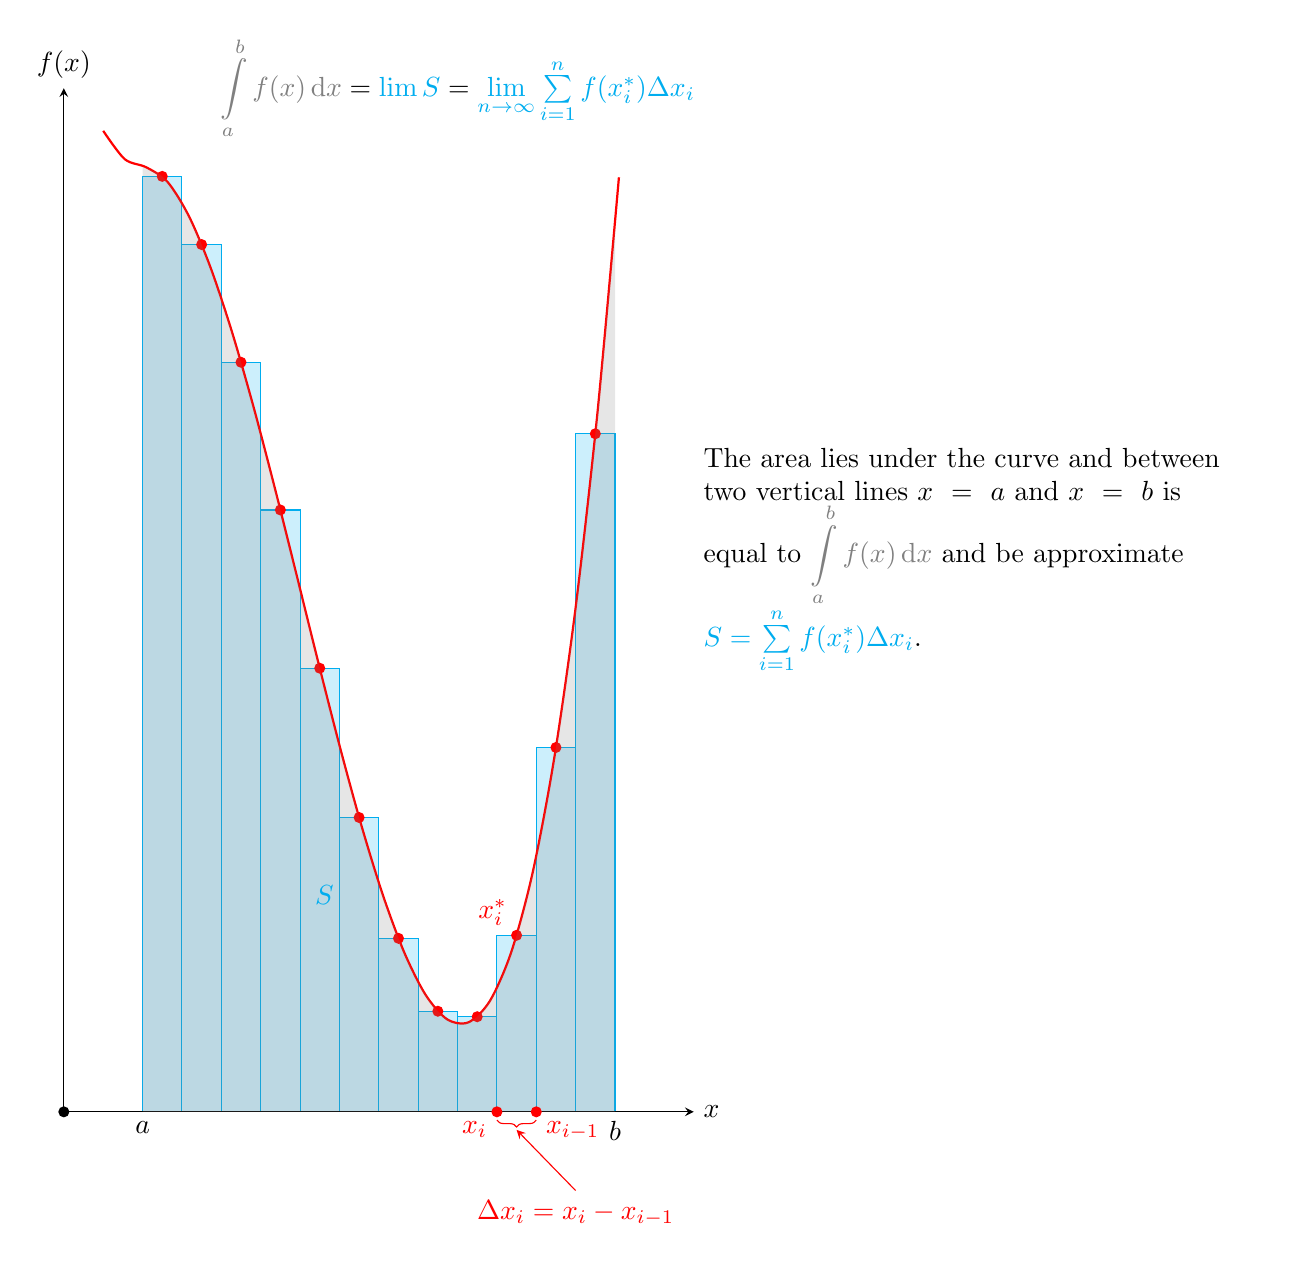
\begin{tikzpicture}
        % draw x-axis and y-axis
        \fill (-1, 0) circle (2pt);
        \draw[-stealth] (-1, 0) -- (7, 0) node[right] {$x$};
        \draw[-stealth] (-1, 0) -- (-1, 13) node[above] {$f(x)$};
        % draw red curve and its particular points
        \draw[thick, red] plot[smooth, domain=-0.5:6.05] (\x, {f(\x)});
        \foreach \x in {0.25, 0.75, 1.25, ..., 6}{
            \fill[color=red] (\x, {f(\x)}) circle (2pt);
        }
        % fill the area (S) lies under the curve and between two vertical lines x=a and x=b
        \fill[gray, fill opacity=0.2] (0, 0) -- (0, {f(0)}) -- plot[smooth, domain=0:6] (\x, {f(\x)}) -- (6, {f(6)}) -- (6, 0) -- cycle;
        % draw cyan rectangles
        \begin{pgfonlayer}{background}
            \foreach \x in {0.25, 0.75, 1.25, ..., 6}{
                \filldraw[fill=cyan!20, draw=cyan] (\x - 0.25, 0) rectangle (\x + 0.25, {f(\x)});
            }
        \end{pgfonlayer}
        % label lower and upper limits (a and b)
        \node[below] at (0, 0) {$a$};
        \node[below] at (6, 0) {$b$};
        % label x_i and x_{i-1} and x*_i
        \fill[red]
            (4.5, 0) node[below left] {$x_i$} circle (2pt)
            (5, 0) node[below right] {$x_{i-1}$} circle (2pt)
            (4.75, {f(4.75)}) node[above left] {$x_i^\ast$};
        % draw brace, \Delta_{x_i} and arrow
        \draw[red, snake=brace, mirror snake, raise snake=3pt] (4.5, 0) -- node (delta_brace) {} (5, 0);
        \node[red, anchor=north] (delta_x) at (5.5, -1) {$\Delta x_{i} = x_{i} - x_{i-1}$};
        \draw[-stealth, red] (delta_x.north) -- ([yshift=-3pt]delta_brace.south);
        % equation
        \node[anchor=center] at (4, 13) {$\textcolor{gray}{\displaystyle\int\limits_a^bf(x)\!\mathop{}\mathrm{d}x} = \textcolor{cyan}{\lim S} = \textcolor{cyan}{\lim\limits_{n\to\infty}\sum\limits_{i=1}^{n}f(x_i^\ast)\Delta x_i}$};
        % add text and area S
        \draw (7, 7) node[right, text width=7cm, black] {
                The area lies under the curve and between two vertical lines $x=a$ and $x=b$ is equal to $\textcolor{gray}{\displaystyle\int\limits_a^bf(x)\!\mathop{}\mathrm{d}x}$ and be approximate $\textcolor{cyan}{S=\sum\limits_{i=1}^{n}f(x_i^\ast)\Delta x_i}$.}
              (2.55, 3) node[below left, cyan] {$S$};
    \end{tikzpicture}
\end{document}